\subsection{Network traffic}
The software for the \textit{programmable end nodes} implementing the required functions is decoupled from the physical node it is deployed on. From a programmers point of view the software is split up un several logical nodes. Each node is responsible for implementing a certain related set of functions examples of logical nodes are: the \textit{Braking System Manager} or the \textit{Lighting Manager}. The logical nodes consist of one or more runnables, the runnable is the smallest software component that is subject to scheduling by the RTOS. This allows to split a logical node in several runnables which can be scheduled independently or deployed on different physical nodes. Runnables communicate with each other through signals, a signal represents a sample of some system state variable. These system state variables can represent a physical value or an abstract value. For example, \textit{brake pedal position} could be a signal generated by a runnable of the \textit{Braking System Manager}, describing the physical position of the brake pedal. While a \textit{Lighting Manager} runnable could consume the \textit{operating mode lighting} signal representing the current state in a state machine. A signal is produced by a single runnable, but can be consumed by multiple runnables. For each logical node a set of deployment files describe which runnables exist, which signals are consumed and produced by each runnable, at what rate the runnables are scheduled and on which \textit{programmable end nodes} they are deployed.

The deployment files are used when building binaries for the \textit{programmable end nodes} to automatically generate code to bridge the required signals between the runnables. First let's consider a pair of runnables consuming/producing the same signal that are deployed on the same \textit{programmable end node}. So one runnable generates a signal while the other is a consumer of that signal. Because the runnables are deployed on the same \textit{programmable end nodes} there is no network traffic necessary. In this case the signal can be thought of as being implemented as a global variable residing in the \textit{programmable end nodes} memory which can be accessed in a thread-safe way by both runnables.

If the producing and consuming runnables are deployed on different \textit{programmable end nodes} which are directly connected to each other e.g, the Vehicle Control Unit and the Central Gateway, the signal has to be transmitted on the network connecting them. In this case the signal is transmitted to the receiving node over CAN at a fixed rate. For efficiency reasons signals that have the same \textit{programmable end node} as destination are packed in the same CAN message.

The last case is when a producing and consuming runnable are deployed on different \textit{programmable end nodes} which are not directly connected to each other e.g, the Vehicle Control Unit and Safety Control Unit. In this case the message has to be bridged across two networks by the Central Gateway. For modelling purposes one can think of having two runnables in the Central Gateway responsible for bridging the data from node A to B. The first being the \textit{gateway\_receive} runnable, which consumes signals from node A. The second being the \textit{gateway\_transmit} runnable, which produces signals for the runnables running on \textit{programmable end node} B, forwarding the consumed signal from the \textit{gateway\_receive} runnable.

Because signals can be consumed by multiple runnables, combinations of the cases mentioned above are possible for a single signal. For example a signal can be consumed by a runnable deployed on the same \textit{programmable end node} and by a runnable on a node without direct CAN connection, requiring bridging by the Central Gateway.

Because the deployment can change as development progresses but also because a deployment is specific to a vehicle type we want to create a description of the data flow on the logical level. This description can be used as an input for generating several deployments whose performance can be evaluated using simulation. The data flow description is specific for a vehicle as it is influenced by the chosen architecture and the feature set. It can serve as a benchmark for a type of vehicle with a known feature set. The data flow description can be adapted to match vehicles with different architectures and feature sets. 

As described earlier the runnables executing on the \textit{programmable end nodes} generate network traffic when signals are shared between runnables on separate nodes. 
\begin{table}[htb]
    \centering
    \resizebox{\textwidth}{!}{%
    \begin{tabular}{@{}llllll@{}}
    \toprule
    signal name  & source physical  & source logical           & destination physical   & destination logical         & data type        \\ \midrule
    active\_gear & scu\_primary     & Vehicle Power Controller & scu\_primary           & Braking System Manager      & int16\_t         \\
    power\_mode  & central\_gateway & VPC Gateway              & scu\_primary           & Vehicle Power Controller    & i\_psm\_state\_t \\
    power\_mode  & central\_gateway & VPC Gateway              & scu\_primary           & Energy Storage Controller   & i\_psm\_state\_t \\
    active\_gear & scu\_primary     & Vehicle Power Controller & scu\_primary           & Gear Selector Manager       & int16\_t         \\
    active\_gear & scu\_primary     & Vehicle Power Controller & scu\_primary           & Safety Supervisor Core      & int16\_t         \\
    power\_mode  & central\_gateway & VPC Gateway              & scu\_primary           & Safety Supervisor Core      & i\_psm\_state\_t \\
    active\_gear & scu\_primary     & Vehicle Power Controller & central\_gateway       & Authentication Manager      & int16\_t         \\
    active\_gear & scu\_primary     & Vehicle Power Controller & central\_gateway       & Media ECU Interface Manager & int16\_t         \\
    active\_gear & scu\_primary     & Vehicle Power Controller & central\_gateway       & Lighting Manager            & int16\_t         \\
    active\_gear & scu\_primary     & Vehicle Power Controller & vehicle\_control\_unit & Driver Controls Manager     & int16\_t         \\
    power\_mode  & central\_gateway & VPC Gateway              & vehicle\_control\_unit & Solar Controller            & i\_psm\_state\_t \\
    power\_mode  & central\_gateway & VPC Gateway              & vehicle\_control\_unit & VPC vcu                     & i\_psm\_state\_t \\ \bottomrule
    \end{tabular}%
    }
    \caption{Interface overview for \textit{power\_mode} and \textit{active\_gear} signals}
    \label{tab:interface_overview}
    \end{table}

\begin{figure}[htb]
    \centering
    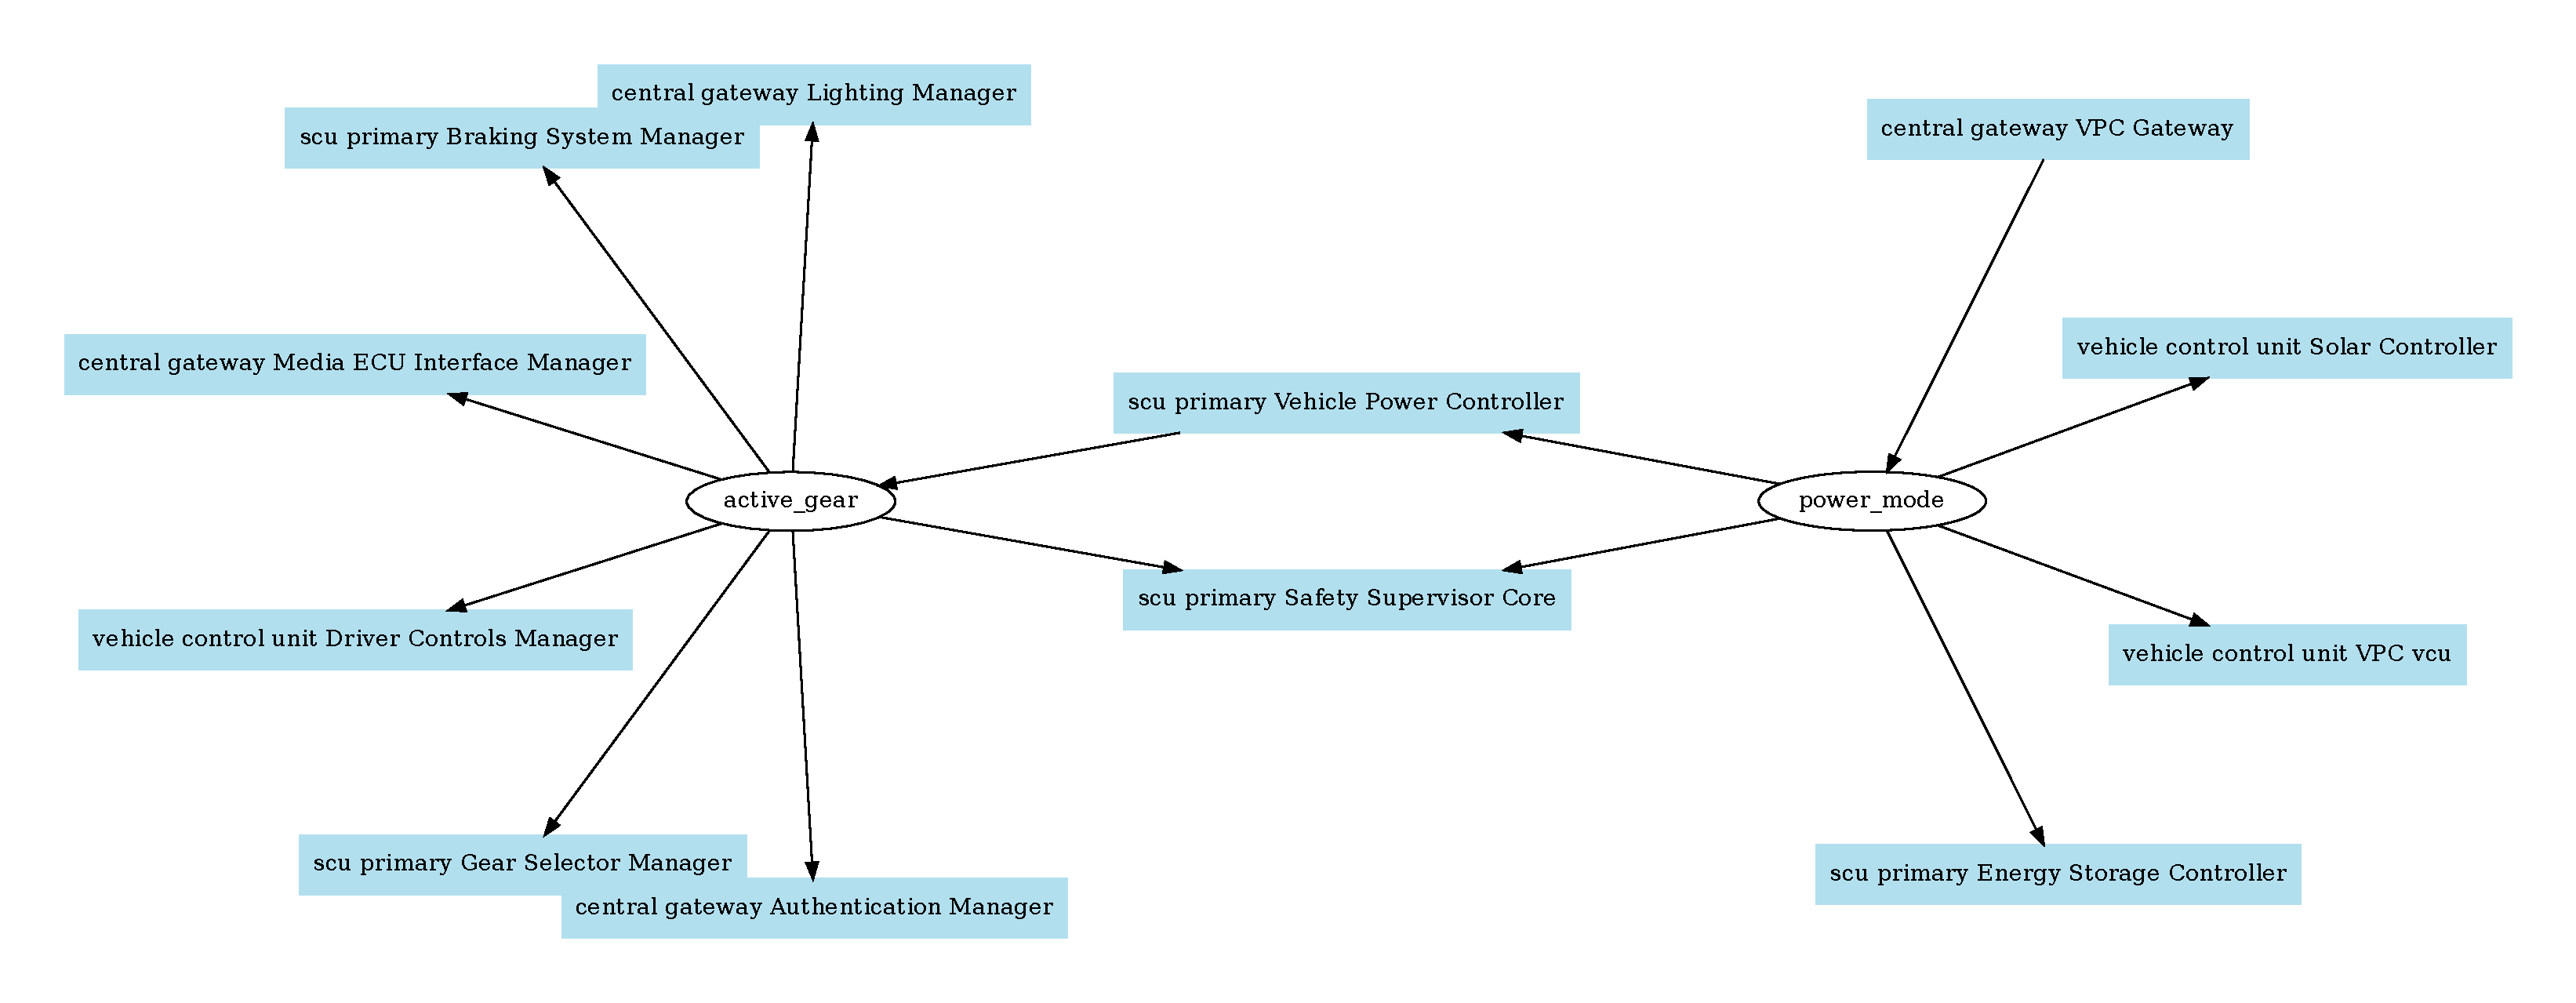
\includegraphics[width=\textwidth]{images/interface_overview.pdf}
    \caption{Interface overview for two signals in graphical form}
    \label{fig:interface_overview}
\end{figure}
\todo{Describe that parametrizable end node traffic is defined in DBC and LDF files, but exact rate is harder to find}
\todo{Describe logging, DTC and update traffic (ISO-TP and UDS)}
\todo{Describe ethernet traffic}